% !TeX program = pdflatex
% Kompilieren mit: pdflatex slides_minimal.tex (zweimal)
%
% Kurzfassung fuer die Betreuerin: nur die Ergebnisse, ein Bild je Folie.
% Text so weit wie moeglich in Formelschreibweise, nie mehr als vier
% Stichpunkte, keine Fliesstextsaetze. Die ausfuehrliche Fassung mit
% Konstruktion, Modellbeschreibung und Einschraenkungen steht in
% slides.tex.
\documentclass[10pt,aspectratio=169]{beamer}

\usetheme{metropolis}

\usepackage[utf8]{inputenc}
\usepackage[T1]{fontenc}
\usepackage{lmodern}
\usepackage[ngerman]{babel}
\usepackage{tikz}
\usepackage{booktabs}
\usepackage{array}
\newcolumntype{L}[1]{>{\raggedright\arraybackslash}p{#1}}
\usepackage{amsmath}

% Gleiche Farben wie die Langfassung, damit beide zusammengehoeren.
\definecolor{giessenblau}{RGB}{28,54,88}
\definecolor{hellblau}{RGB}{230,234,240}
\definecolor{grauton}{RGB}{95,102,110}
\definecolor{hellgrau}{RGB}{236,236,237}

\setbeamercolor{palette primary}{bg=giessenblau,fg=white}
\setbeamercolor{frametitle}{bg=white,fg=giessenblau}
\setbeamercolor{progress bar}{fg=giessenblau,bg=giessenblau!20}
\setbeamercolor{alerted text}{fg=giessenblau}
\setbeamertemplate{itemize item}{\color{giessenblau}\textbullet}
\setbeamercolor{block title}{bg=giessenblau,fg=white}
\setbeamercolor{block body}{bg=hellblau}
\setbeamercolor{block title alerted}{bg=grauton,fg=white}
\setbeamercolor{block body alerted}{bg=hellgrau,fg=black}

\metroset{sectionpage=none, numbering=fraction, progressbar=frametitle}
\makeatletter
\setlength{\metropolis@progressinheadfoot@linewidth}{2pt}
\makeatother

% Listen etwas straffer als beamers Standard.
\makeatletter
\let\jlu@olditemize\itemize
\let\jlu@oldenditemize\enditemize
\renewenvironment{itemize}
  {\jlu@olditemize\setlength{\itemsep}{4pt}\setlength{\parsep}{0pt}\setlength{\topsep}{2pt}}
  {\jlu@oldenditemize}
\makeatother

\newcommand{\hinweis}[1]{{\scriptsize\color{grauton} #1}}
\newcommand{\vortragsdatum}{07.11.2026}

\title{RFN: Frequenzvariation}
\author{Konrad Wehkamp}
\date{}

\begin{document}

% ============================================================
{
\setbeamertemplate{footline}{}
\begin{frame}[plain,c]
  \begin{tikzpicture}[remember picture, overlay]
    \node[anchor=north west, inner sep=0pt] at ([xshift=0.9cm,yshift=-0.6cm]current page.north west)
      {
\includegraphics[height=1.0cm]{img/JLU_Giessen-Logo.pdf}};
    \draw[giessenblau, line width=0.8pt] ([yshift=-1.7cm]current page.north west) -- ([yshift=-1.7cm]current page.north east);
    \draw[giessenblau, line width=0.8pt] ([yshift=1.6cm]current page.south west) -- ([yshift=1.6cm]current page.south east);
  \end{tikzpicture}
  \begin{center}
    {\LARGE\bfseries\color{giessenblau} RFN: Frequenzvariation 2 bis 40\,MHz}\\[0.7em]
    {\Large\color{grauton} Ergebnisse der COMSOL-Rechnung}\par
    \vspace{1.0cm}
    {\large Konrad Wehkamp}\\[0.3em]
    {\small\color{grauton} \vortragsdatum}
  \end{center}
\end{frame}
}

% ============================================================
\begin{frame}{Modell}
  \vfill
  \begin{align*}
    P_\mathrm{ohm}  &= (1-\eta_k)\,P_\mathrm{in} \\[0.2em]
    P_\mathrm{wand} &= \eta_k\,f_\mathrm{wand}\,P_\mathrm{in} \\[0.2em]
    I_\mathrm{Spule} &= I_\mathrm{ref}\sqrt{P_\mathrm{ohm}/P_\mathrm{met,ref}}
  \end{align*}
  \vspace{0.3em}
  \begin{itemize}
    \item Magnetfeld $+$ Wärmetransport $+$ Oberflächenstrahlung, gekoppelt
    \item Plasma als Drude-Leitfähigkeit, $p = 0{,}02$\,mbar
    \item $P_\mathrm{in} = 150$\,W, $f_\mathrm{wand} = 0{,}22$, Aluminium-Unterring
  \end{itemize}
  \vfill
\end{frame}

% ============================================================
\begin{frame}{Kopplungsgrad: $\eta_k = 75\,\% \rightarrow 94\,\%$}
  \centering
  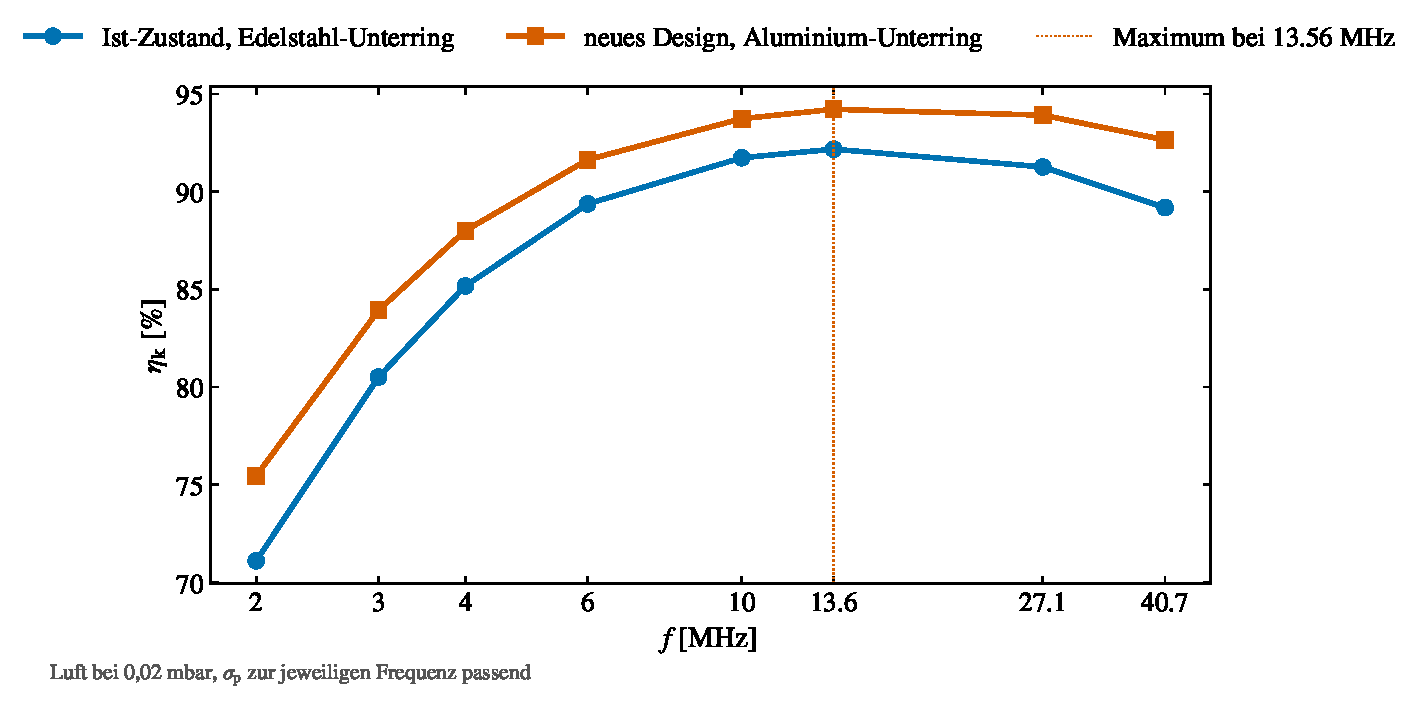
\includegraphics[height=6.4cm]{img/abb01_kopplungsgrad.pdf}
\end{frame}

% ============================================================
\begin{frame}{Restverlust: $P_\mathrm{ohm} = 36{,}8 \rightarrow 8{,}7 \rightarrow 11{,}0\,$W}
  \centering
  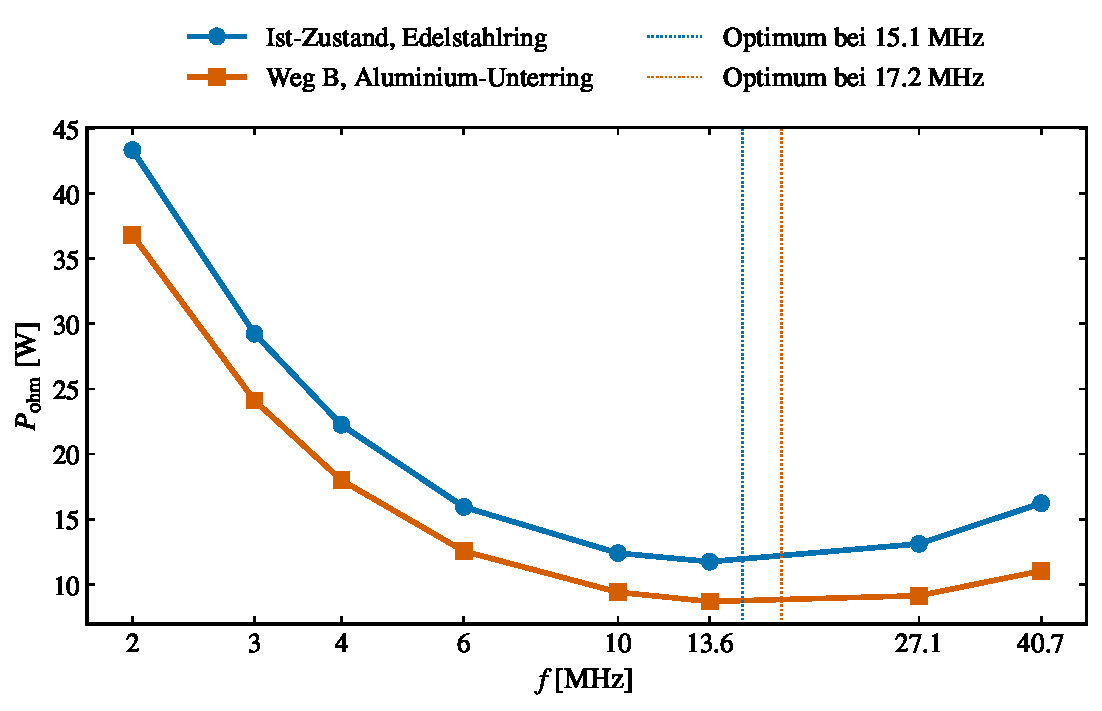
\includegraphics[height=6.4cm]{img/abb02_restverlust.pdf}
\end{frame}

% ============================================================
\begin{frame}{Optimum}
  \vfill
  \[
    \omega_\mathrm{opt} = \nu_m\sqrt{\frac{2-\alpha}{\alpha}},
    \qquad \alpha = 0{,}463 \ \text{(gemessen)}
  \]
  \vspace{0.2em}
  \begin{itemize}
    \item $f_\mathrm{opt} = 16{,}6$\,MHz aus der Formel, 15,1\,MHz aus den acht Punkten
    \item LXCat, $T_e = 4{,}5$\,eV: $f_\mathrm{opt} = 14{,}5$ bis $19$\,MHz
    \item $f_\mathrm{opt} \propto p$, unabhängig von $n_e$ und Spulengeometrie
  \end{itemize}
  \vfill
\end{frame}

% ============================================================
\begin{frame}{$R_\mathrm{Plasma}$ sättigt, $R_\mathrm{Metall} \propto \omega^{0{,}463}$}
  \centering
  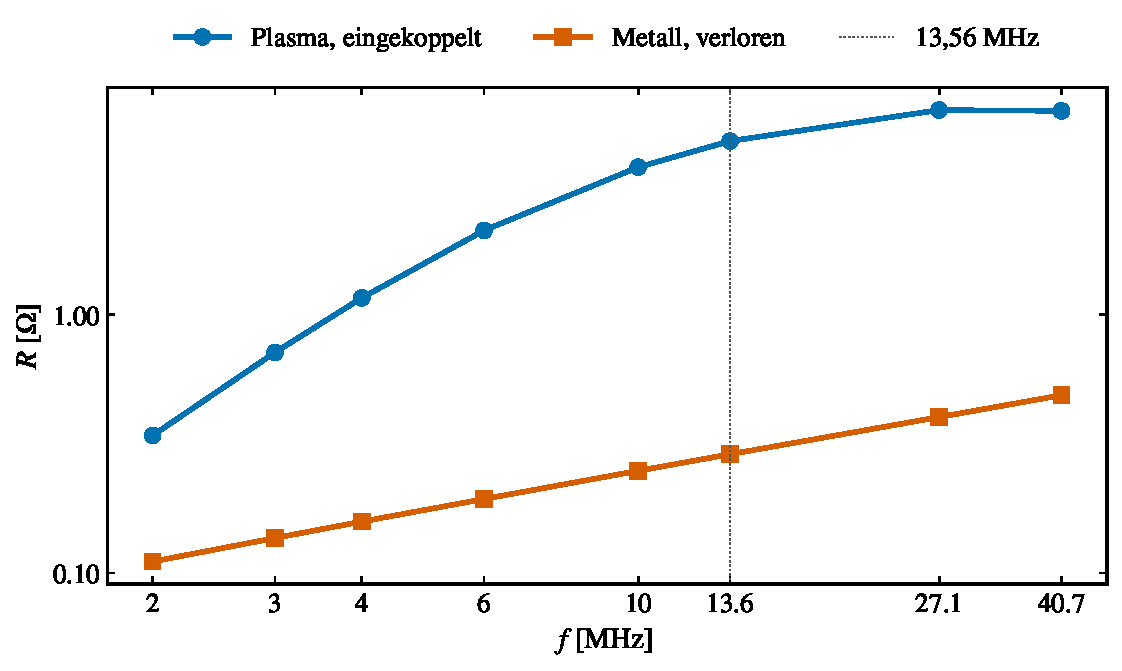
\includegraphics[height=6.4cm]{img/abb13_widerstaende.pdf}
\end{frame}

% ============================================================
% Das Balkendiagramm ist flacher als die Kurvenbilder und fuellt die Folie
% nicht von selbst. Ueber die Breite statt die Hoehe einpassen und mit
% \vfill zentrieren, sonst haengt es oben und laesst unten eine Luecke.
\begin{frame}{Verlustaufteilung bei 4\,MHz}
  \vfill
  \centering
  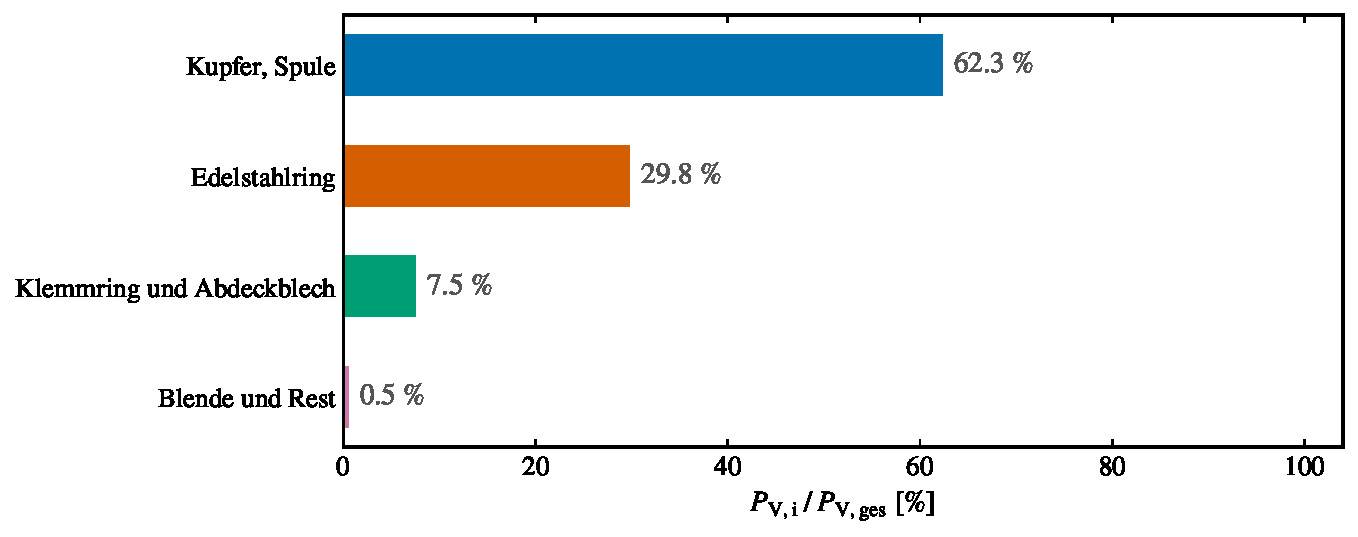
\includegraphics[width=\linewidth]{img/abb05_verlustaufteilung.pdf}

  \vspace{0.8em}
  \hinweis{Bei 40,68\,MHz trägt der Unterring allein rund 45\,\%.}
  \vfill
\end{frame}

% ============================================================
\begin{frame}{Temperaturen bei 4\,MHz und 150\,W}
  \centering
  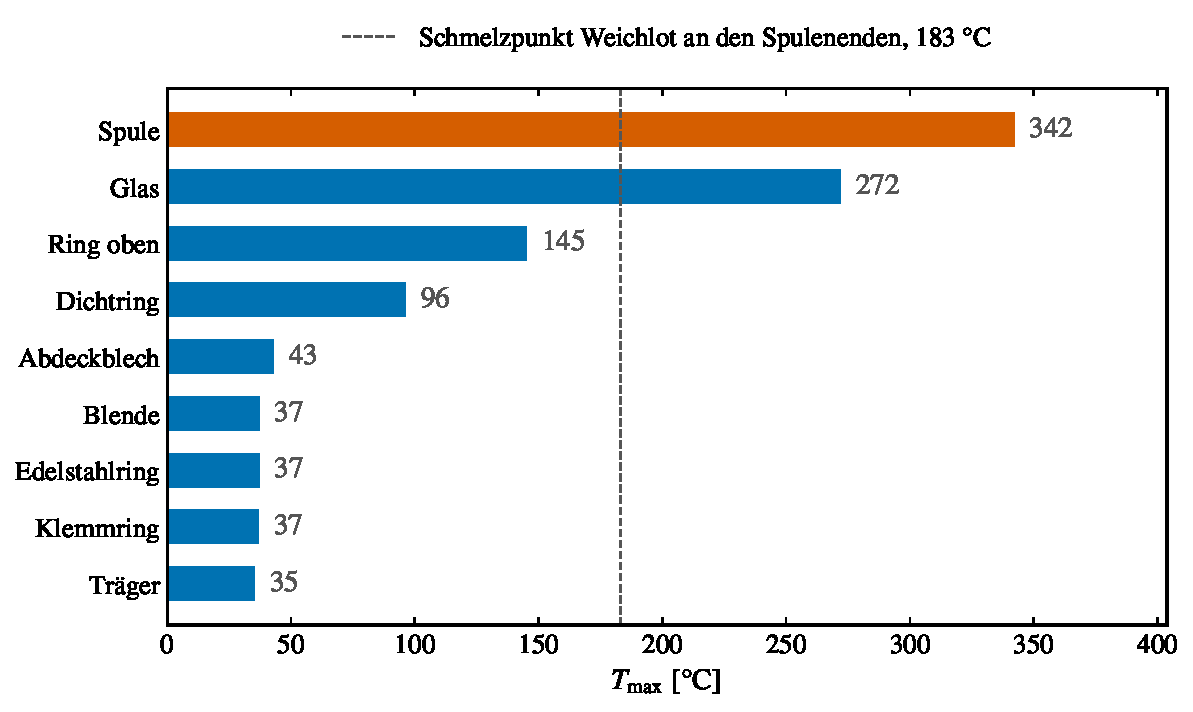
\includegraphics[height=6.4cm]{img/abb06_temperaturen.pdf}
\end{frame}

% ============================================================
\begin{frame}{$T_\mathrm{Spule} = 445 \rightarrow 267 \rightarrow 303\,^\circ$C}
  \centering
  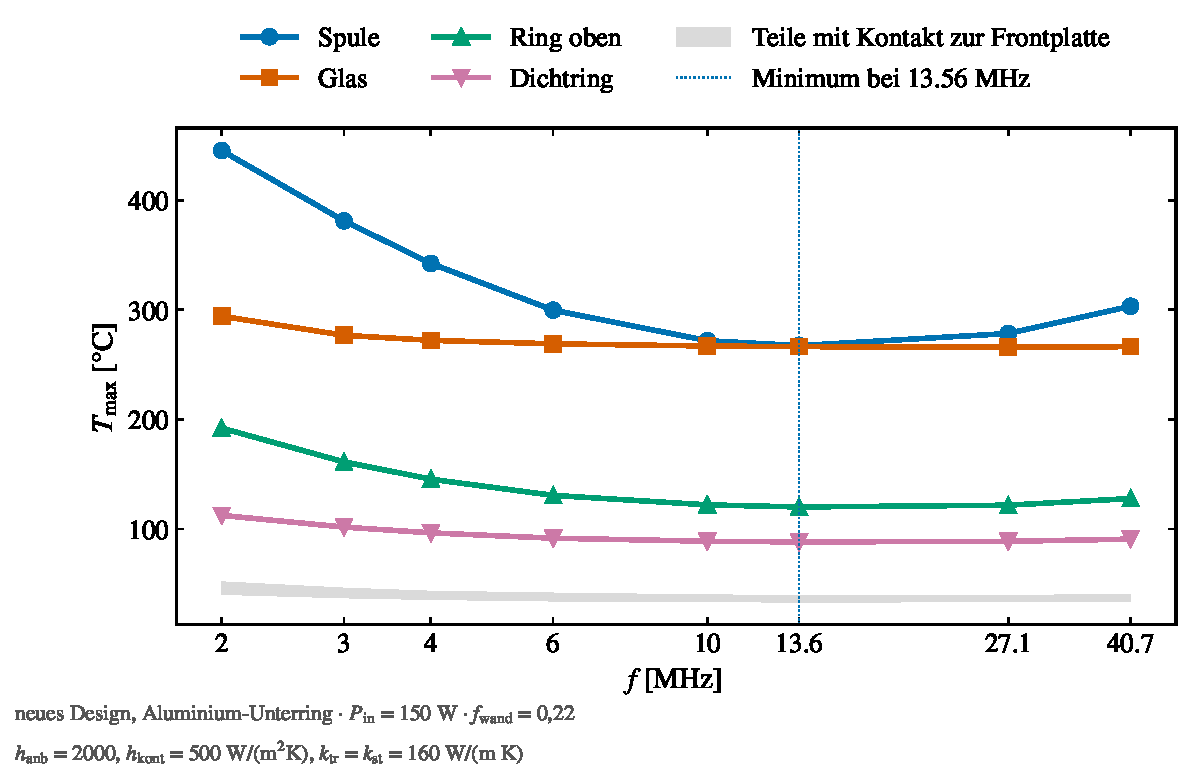
\includegraphics[height=6.4cm]{img/abb10_temperatur_ueber_frequenz.pdf}
\end{frame}

% ============================================================
\begin{frame}{Betriebskarte: farbig $f$, grau $P_\mathrm{in}$}
  \centering
  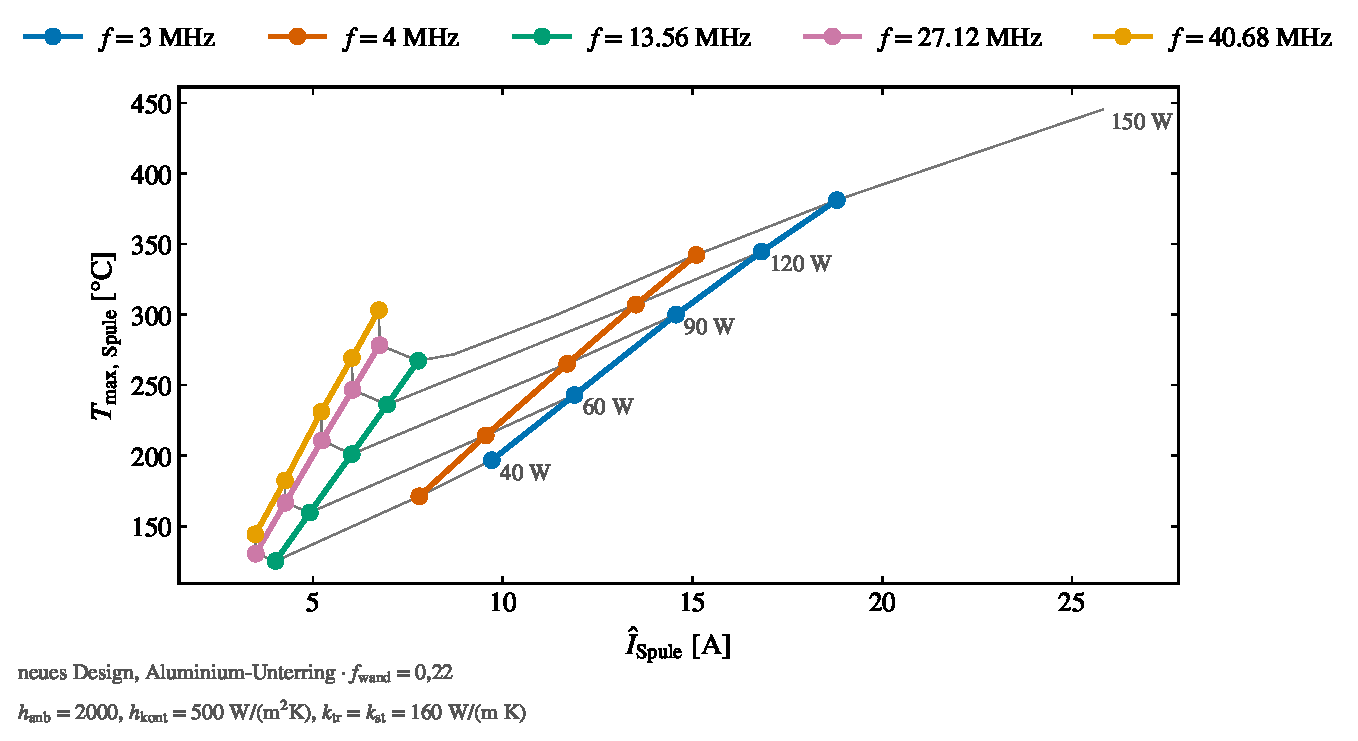
\includegraphics[height=6.4cm]{img/abb14_betriebskarte.pdf}
\end{frame}

% ============================================================
\begin{frame}{Gegenprobe: $P_\mathrm{Plasma}$ geregelt, Optimum bleibt}
  \centering
  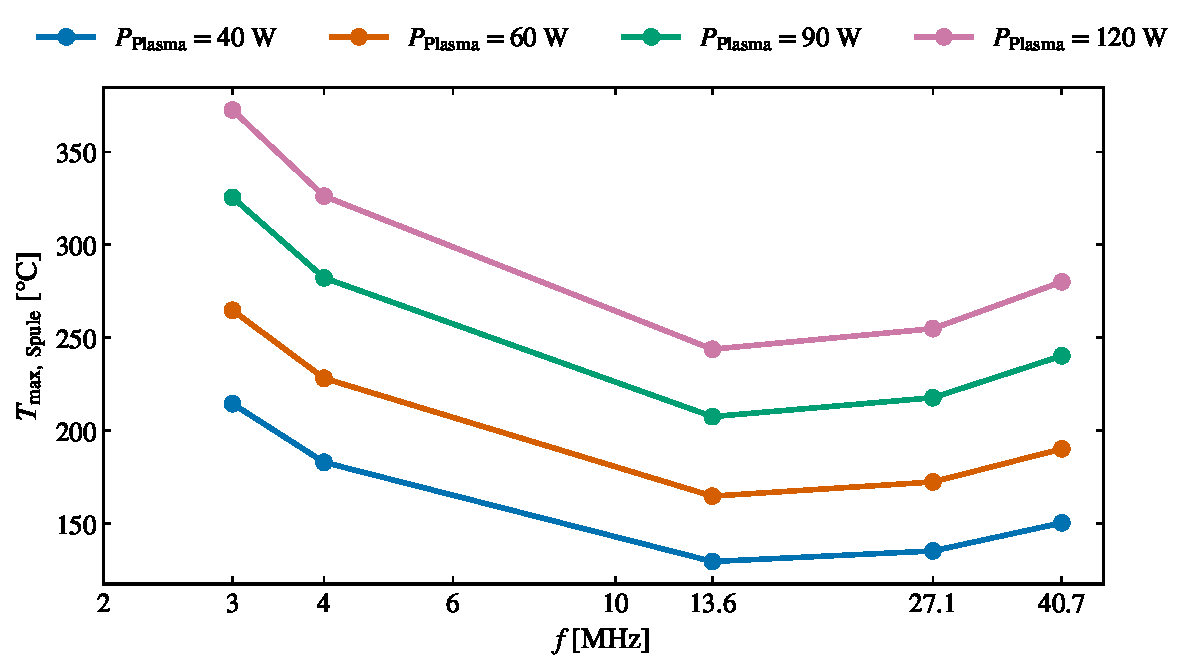
\includegraphics[height=6.4cm]{img/abb15_regelung_plasmaleistung.pdf}
\end{frame}

% ============================================================
\begin{frame}{Modellgüte}
  \vfill
  \begin{itemize}
    \item Schließprobe $P_\mathrm{Cu} + P_\mathrm{R\ddot{a}nder}$ gegen $P_\mathrm{ohm}$: max.\ $0{,}034\,\%$
    \item Bilanzprobe $\sum P$ gegen $P_\mathrm{in}$: max.\ $0{,}058\,\%$
    \item $\eta_k$ zurückgerechnet: $0{,}87999$ gegen $0{,}88000$ vorgegeben
    \item Netzstudie: Proximity-Faktor $2{,}28 \pm 0{,}05$, \ $L = 1{,}47\,\mu$H
  \end{itemize}
  \vfill
\end{frame}

% ============================================================
\begin{frame}{Offen}
  \vfill
  \begin{itemize}
    \item $h_\mathrm{anb} = 2000\ \mathrm{W/(m^2K)}$ angesetzt, nicht gemessen
    \item $\sigma_p$ über die Leistungsleiter konstant, $n_e(P)$ fehlt
    \item Kapazitive Einkopplung nicht modelliert
    \item Eichregularisierung im Vakuum: Test läuft, Teilleistungen nicht betroffen
    \item Edelstahl-Reihe besteht die Schließprobe nicht
  \end{itemize}
  \vfill
\end{frame}

% ============================================================
\begin{frame}{Fragen}
  \vfill
  \begin{itemize}
    \item Festfrequenzen der neuen RFGs?
    \item Betriebsdruck? \ $f_\mathrm{opt} \propto p$
    \item Gaszusammensetzung? Gerechnet N$_2$/O$_2$ $=$ 79/21
    \item Aluminium-Variante bauen?
  \end{itemize}
  \vfill
\end{frame}

% ============================================================
{
\setbeamertemplate{footline}{}
\begin{frame}[plain,c]
  \begin{tikzpicture}[remember picture, overlay]
    \node[anchor=north west, inner sep=0pt] at ([xshift=0.9cm,yshift=-0.6cm]current page.north west)
      {
\includegraphics[height=1.0cm]{img/JLU_Giessen-Logo.pdf}};
    \draw[giessenblau, line width=0.8pt] ([yshift=-1.7cm]current page.north west) -- ([yshift=-1.7cm]current page.north east);
    \draw[giessenblau, line width=0.8pt] ([yshift=1.6cm]current page.south west) -- ([yshift=1.6cm]current page.south east);
  \end{tikzpicture}
  \begin{center}
    {\LARGE\bfseries\color{giessenblau} $f_\mathrm{opt} \approx 15\,$MHz}\\[0.8em]
    {\Large\color{grauton} von den Festfrequenzen also 13,56\,MHz}
  \end{center}
\end{frame}
}

\end{document}
